\documentclass[conference]{IEEEtran}
\IEEEoverridecommandlockouts
% The preceding line is only needed to identify funding in the first footnote. If that is unneeded, please comment it out.
\usepackage{cite}
\usepackage{amsmath,amssymb,amsfonts}
\usepackage{algorithmic}
\usepackage{graphicx}
% \usepackage{natbib}
% \usepackage{textcomp}
\usepackage{xcolor}
\usepackage{subfig}
\usepackage{float}
\usepackage{lipsum}
\usepackage{longtable}
\usepackage{verbatim}
% \usepackage{times} % assumes new font selection scheme installed
\setlipsum{%
  par-before = \begingroup\color{gray},
  par-after = \endgroup
}
\usepackage{hyperref}
% \def\BibTeX{{\rm B\kern-.05em{\sc i\kern-.025em b}\kern-.08em
%     T\kern-.1667em\lower.7ex\hbox{E}\kern-.125emX}}

\def\aj{\textit{AJ}}                   % Astronomical Journal
\def\apj{\textit{ApJ}}                 % Astrophysical Journal
\def\apjs{\textit{ApJS}}               % Astrophysical Journal, Supplement
\let\apjlett=\apjl
\def\mnras{\textit{MNRAS}}             % Monthly Notices of the RAS
\def\pasp{\textit{PASP}}               % Publications of the ASP

\newtheorem{defn}{Definition}[section]
\newtheorem{cor}{Corollary}
\newtheorem{exmp}{Example}[section]
\renewcommand\thecor{\unskip}
\renewcommand\theexmp{\unskip}


\title{\LARGE \bf
Light curve classification using distance metrics
}

\begin{document}
\bstctlcite{IEEEexample:BSTcontrol}

\author{\IEEEauthorblockN{Siddharth Chaini\IEEEauthorrefmark{1}\IEEEauthorrefmark{2}\thanks{Corresponding author: S. Chaini (\href{mailto:sidchaini@gmail.com}{sidchaini@gmail.com}).},
Ashish Mahabal\IEEEauthorrefmark{3}\IEEEauthorrefmark{4},
Federica Bianco\IEEEauthorrefmark{2}, 
Ajit Kembhavi\IEEEauthorrefmark{5}, and
Sukanta Panda\IEEEauthorrefmark{1}}
\IEEEauthorblockA{\IEEEauthorrefmark{1}Department of Physics, Indian Institute of Science Education and Research, Bhopal 462066, India}
\IEEEauthorblockA{\IEEEauthorrefmark{2}Department of Physics and Astronomy, University of Delaware, Newark, DE 19716-2570, USA}
\IEEEauthorblockA{\IEEEauthorrefmark{3}Division of Physics, Mathematics and Astronomy, California Institute of Technology, Pasadena, CA 91125, USA}
\IEEEauthorblockA{\IEEEauthorrefmark{4}Center for Data Driven Discovery, California Institute of Technology, Pasadena, CA 91125, USA}
\IEEEauthorblockA{\IEEEauthorrefmark{5}Inter University Centre for Astronomy and Astrophysics (IUCAA), Pune 411007, India}
% <-this % stops an unwanted space
}

\maketitle

\begin{abstract}
The rise of extensive sky surveys has ushered in an era of big data in time-domain astronomy, which has made data science and machine learning an essential tool for classification. In this paper, we present the use of distance metrics for classification of light curves. In particular, we classify light curves of variable stars by comparing the distances between objects of different classes.
A distance is an abstract quantity that tells us about the closeness of two objects, and a distance metric is a rule to calculate this distance. We demonstrate the use of various distance metrics for the dimensionality reduction and classification of light curves and compare the performance of different distance metrics for different classes.
We find that certain classes and features are easier to separate with specific metrics. The use of different distance metrics for classification and dimensionality reduction is an approach that has not been explored in time-domain astronomy yet.
\end{abstract}

\begin{IEEEkeywords}
some, keywords
\end{IEEEkeywords}

\section{Introduction}
Over the last few decades, time-domain astrophysics has experienced rapid growth. The significant factors behind this growth have been the advent of large-scale sky surveys like the Sloan Digital Sky Survey (SDSS; \cite{yorkSloanDigitalSky2000}), the Catalina Real-Time Transient Survey (CRTS; \cite{djorgovskiCatalinaRealTimeTransient2011}) and the Zwicky Transient Facility (ZTF;\cite{bellmZwickyTransientFacility2019}) (See \cite{Djorgovski2013} for more surveys.) accompanied by advances in computer data storage. By observing how millions of astronomical objects change over time, we can look at changes in the night sky that were once impossible to detect. The Rubin Observatory Legacy Survey of Space and Time (LSST;\cite{ivezicLSSTScienceDrivers2019}), is expected to observe over 37 billion objects over its 10-year lifespan. However, this opportunity for new discoveries in the data deluge is accompanied by a data-intensive challenge. Manual human classification of all objects has become impossible, and we need to deploy methods that can automate the classification and identification of objects of interest. Machine learning is one such approach to it.

Machine learning refers to a class of computer algorithms in which the computer automatically learns patterns from data without being programmed. Thus, in the context of the big datasets and the need for automation, machine learning has become essential in modern astrophysics. One such machine learning task which is critical to time-domain astrophysics is the classification of astronomical objects based on how their brightness changes with time
% (called light curves; formally introduced in Section \ref{subsec:light_curves})
. Machine learning for this involves extracting features from the light curves, which are then fed to the machine learning algorithm. However, as the number of features used in a machine learning model increases, prediction becomes difficult and computationally expensive. This complexity is mainly because of the ``curse of dimensionality" \cite{bishopPatternRecognitionMachine2006}, which leads to a decrease in performance and an increase in computational complexity. Furthermore, this is accompanied by data abstraction, which results in the model behaving like a black-box, and makes explainability difficult.

To help tackle the above problems, we can reduce dimensionality by transforming our data. This involves mapping our data from a high dimensional space into a low dimensional space while ensuring that the low dimensional representation retains the properties of the original data.

A distance is a scalar quantity that tells us how far away two objects are, while a distance metric refers to the method by which this distance is calculated. Because the distance between objects from the same class is smaller than objects from different classes, an analysis of these distances can be used to separate and classify light curves.

In this paper, we compare the use of different distance metrics to classify light curves and reduce the dimensionality of their feature space. We look at 18 different metrics and compare their performance for different types of classification problems for variable stars. In addition, we also find the most important features associated with a particular distance metric and reduce the dimensionality of the feature space to these top features. The use of different distance metrics in this goal is an approach that has not been explored in time-domain astrophysics yet.

The paper is organised as follows: % We introduce some of the scientific and technical background in Chapter \ref{chap:background}, then talk about our methodology behind the classification and dimensionality reduction in Chapter \ref{chap:methods}, then present our results in Chapter \ref{chap:results} and finally conclude with future work and discussion in Chapter \ref{chap:conclusion}.


\section{Distances in Machine Learning}
The notion of distance is intuitive to most of us. It tells us about the degree of closeness of two physical objects or ideas. The shorter the distance, the closer the objects or ideas are. However, the existence of such a quantity does not tell us how to calculate it. Because of this, we can have different types of distances, each calculated differently. These distances can have different physical meanings, but they can also be entirely abstract. A formal definition has been listed in \ref{}

For most machine learning tasks, we cannot feed the data directly to the machine learning model. For this reason, we generally extract \emph{features} from the training data and transform it into a new space called the feature space. The dimensionality of the feature space is the number of features (columns of the data) we extract from the training data, and the feature space forms the metric space. The points in this space are given by the individual data points (rows of the data). The feature space is similar to the n-dimensional real coordinate space, $\mathbb{R}^n$.

Now, we can define a variety of distance metrics in this higher dimensional feature space, as per definition \ref{def:distance}. Because the distance is always a positive real number, it can be compared easily for different points even if the feature space is highly dimensional.

Distance metrics see their use in a variety of machine learning algorithms, in both supervised (for e.g., k-Nearest Neighbours; \cite{abualfeilatEffectsDistanceMeasure2019}) and unsupervised settings (for e.g., kernel density estimation; \cite{heKernelDensityMetric2013}). We have listed each distance metric that we use in \ref{app:list_of_metrics}.

\section{Data} \label{sec:data}
\subsection{Catalog and Raw Light Curves} \label{subsec:catalog}
To develop our methodology for light curve classification with distance metrics, we choose to work only with variable stars. However, because the only input to our model consists of light curves, we note that our methodology is transferable to light curves of all variables as well as transient classes.

Our raw dataset consists of light curves from the Zwicky Transient Facility (ZTF). To select variable stars, we use the classifications from the catalog provided by \cite{chenZwickyTransientFacility2020a}, which is based on the ZTF Data Release 2 (DR2). The catalog consists of a total of 781,602 identified variable stars. However, the number of objects in each class is imbalanced, with the catalog containing 369,707 EW variables, but just 1,262 Cepheid variables. This forms an imbalanced dataset, as each class has an unequal number of objects. One of the issues with imbalanced classification problems is that models trained on an imbalanced dataset have a hidden bias due to the relative frequencies when the machine learns from the data and perform poorly on minority classes \cite{krawczykLearningImbalancedData2016}. Thus, we choose only 1,000 objects of each class from \cite{chenZwickyTransientFacility2020a}'s dataset to work with a balanced number of classes throughout this thesis.

Our raw dataset thus consists of 100,000 light curves (10,000 for each of the 10 classes listed in Tab. \ref{tab:variable_summary}). We download these from the catalog website\footnote{\href{http://variables.cn:88}{http://variables.cn:88}}.

\subsection{Feature Extraction} \label{subsec:feature_extraction}
Since the ZTF is a ground-based telescope, the light curves obtained are sparse and unevenly sampled, noisy and heteroskedastic. On top of that, even objects belonging to the same classes have different noise levels and different magnitudes based on their distance from the earth. Because of this, the direct comparison of light curves is difficult. However, we can instead extract different features from these light curves - attributes that give us some information about the light curve. These features allow us to compare different light curves better and are fed to the machine learning algorithm for classification.


To extract features from the light curves, we use the \texttt{lc\_classifier} module \cite{jainagaAlercebrokerLcClassifier2021} on Python. All of \texttt{lc\_classifier}'s features are based on the light curves only. Most (50) features are calculated separately for the g and r passband, while some (8) features are calculated using both the g and r observations. In addition to this, we also use 5 features for each passband provided by \cite{chenZwickyTransientFacility2020a}. This gives us a total of 118 features for every light curve in our dataset.

Most features are based on the light curve statistics (e.g. \texttt{Amplitude} - based on the difference of highest and lowest magnitudes), while a few are based on parameters obtained after fitting a model (e.g. \texttt{Multiband\_Period} - the period is obtained by fitting a periodogram). A list of all the features, along with their descriptions, is
% given in Tab. \ref{tab:alercefeatures}. A detailed description of all features is
available in Section 3.1 and Appendix A of \cite{sanchez-saezAlertClassificationALeRCE2021}.

% % \clearpage
% \onecolumn
% \begin{longtable}[l]{p{2.5cm}p{7cm}p{3cm}}
%     \caption{List of all light curve features extracted by \texttt{lc\_classifier}. This table has been reproduced from Table 2, \cite{sanchez-saezAlertClassificationALeRCE2021}. An interactive online version is available \href{https://siddharthchaini.github.io/redirects/lcdm_features.html}{here}.} \label{tab:alercefeatures} \\
%     \hline
%     \hline
%     Feature & Description & Reference\\
%     \hline
%     \texttt{delta\_period} & Absolute value of the difference between the \texttt{Multiband\_period} and the MHAOV period obtained using a single band & \cite{sanchez-saezAlertClassificationALeRCE2021} \\
%     \texttt{IAR\_phi} & Level of autocorrelation using a  discrete-time representation of a DRW model & \cite{eyheramendyIrregularDiscreteTime2018}\\
%     MHPS parameters & Obtained from a MHPS analysis (three in total) & \cite{arevaloMexicanHatHoles2012} \\
%     \texttt{Power\_rate}  & Ratio between the power of the multiband periodogram obtained for the best  period candidate ($P$) and $2\times P$, $3\times P$, $4\times P$, $P/2$, $P/3$ or $P/4$ & \cite{sanchez-saezAlertClassificationALeRCE2021} \\
%     \texttt{PPE}  & Multiband Periodogram Pseudo Entropy & \cite{sanchez-saezAlertClassificationALeRCE2021} \\
%     \hline
%     \texttt{ExcessVar} & Measure of the intrinsic variability amplitude & \cite{allevatoMEASURINGXRAYVARIABILITY2013}\\
%     \texttt{GP\_DRW\_tau} & Relaxation time $\tau$ from DRW modeling & \cite{grahamUnderstandingExtremeQuasar2017}\\
%     \texttt{GP\_DRW\_sigma} & Amplitude of the variability at short timescales ($t << \tau$), from DRW modeling & \cite{grahamUnderstandingExtremeQuasar2017}\\
%     Harmonics parameters & Obtained by fitting a harmonic series up to the seventh harmonic (14 in total) & \cite{stellingwerfFourierCoefficientsVariable1986} \\
%     \texttt{Multiband\_ period}  & Period obtained using the multiband MHAOV periodogram & \cite{mondrikMULTIBANDGENERALIZATIONMULTIHARMONIC2015}\\
%     \texttt{Pvar} & Probability that the source is intrinsically variable & \cite{mclaughlinVariabilityCGROEGRET1996}\\
%     \texttt{SF\_ML\_ amplitude}& rms magnitude difference of the SF, computed over a 1 yr timescale &  \cite{schmidtSELECTINGQUASARSTHEIR2010} \\
%     \texttt{SF\_ML\_gamma} & Logarithmic gradient of the mean change in magnitude &  \cite{schmidtSELECTINGQUASARSTHEIR2010} \\
%     \hline
%     \texttt{Amplitude} & Half of the difference between the median of the maximum 5\% and of the minimum 5\% magnitudes & \cite{richardsMACHINELEARNEDCLASSIFICATIONVARIABLE2011}\\
%     \texttt{Anderson- Darling} & Test of whether a sample of data comes from a population with a specific distribution & \cite{nunFATSFeatureAnalysis2015}\\
%     \texttt{Autocor\_ length} & Lag value where the auto-correlation function becomes smaller than \texttt{Eta\_e} & \cite{kimQUASISTELLAROBJECTSELECTION2011}\\
%     \texttt{Beyond1Std} & Percentage of points with photometric mag that lie beyond 1$\sigma$ from the mean & \cite{richardsMACHINELEARNEDCLASSIFICATIONVARIABLE2011}\\
%     \texttt{Con} & Number of three consecutive data points brighter/fainter than 2$\sigma$ of the light curve & \cite{kimQUASISTELLAROBJECTSELECTION2011}\\
%     \texttt{Eta\_e} & Ratio of the mean of the squares of successive mag differences to the variance of the light curve& \cite{kimEPOCHProjectPeriodic2014}\\
%     \texttt{Gskew} & Median-based measure of the skew & \cite{nunFATSFeatureAnalysis2015}\\
%     \texttt{LinearTrend} & Slope of a linear fit to the light curve & \cite{richardsMACHINELEARNEDCLASSIFICATIONVARIABLE2011}\\
%     \texttt{MaxSlope} & Maximum absolute magnitude slope between two consecutive observations & \cite{richardsMACHINELEARNEDCLASSIFICATIONVARIABLE2011}\\
%     \texttt{Meanvariance} & Ratio of the standard deviation to the mean magnitude & \cite{nunFATSFeatureAnalysis2015}\\
%     \texttt{MedianAbsDev} & Median discrepancy of the data from the median data & \cite{richardsMACHINELEARNEDCLASSIFICATIONVARIABLE2011}\\
%     \texttt{MedianBRP} & Fraction of photometric points within amplitude/10 of the median mag & \cite{richardsMACHINELEARNEDCLASSIFICATIONVARIABLE2011}\\
%     \texttt{PairSlope- Trend} & Fraction of increasing first differences minus fraction of decreasing first differences over the last 30 time-sorted mag measures & \cite{richardsMACHINELEARNEDCLASSIFICATIONVARIABLE2011}\\
%     \texttt{Percent- Amplitude} & Largest percentage difference between either max or min mag and median mag & \cite{richardsMACHINELEARNEDCLASSIFICATIONVARIABLE2011}\\
%     \texttt{Psi\_CS} & Range of a cumulative sum applied to the phase-folded light curve & \cite{kimQUASISTELLAROBJECTSELECTION2011}\\
%     \texttt{Psi\_eta} & \texttt{Eta\_e} index calculated from the folded light curve & \cite{kimEPOCHProjectPeriodic2014}\\
%     \texttt{Q31} & Difference between the 3\textsuperscript{rd} and the 1\textsuperscript{st} quartile of the light curve & \cite{kimEPOCHProjectPeriodic2014}\\
%     \texttt{Rcs} & Range of a cumulative sum & \cite{kimQUASISTELLAROBJECTSELECTION2011}\\
%     \texttt{Skew} & Skewness measure & \cite{richardsMACHINELEARNEDCLASSIFICATIONVARIABLE2011}\\
%     \texttt{Small- Kurtosis} & Small sample kurtosis of the magnitudes & \cite{richardsMACHINELEARNEDCLASSIFICATIONVARIABLE2011}\\
%     \texttt{Std} & Standard deviation of the light curve & \cite{nunFATSFeatureAnalysis2015}\\
%     \texttt{StetsonK} & Robust kurtosis measure & \cite{kimQUASISTELLAROBJECTSELECTION2011}\\
%     \hline
%     \hline
% \end{longtable}
% % \clearpage
% \twocolumn

\subsection{Data Cleaning} \label{subsec:data_cleaning}
To clean our dataset, we first start by removing those objects from our dataset for which feature extraction with \texttt{lc\_classifier} failed - thus removing all objects for which even a single feature was not calculated. For most classes, the number of such objects are 3-8\%, but we find that the classes Mira, CEP and SR have a higher fit failure rate, thus leaving us with only 640 Miras, 713 CEPs and 741 SRs . However, to keep the dataset balanced, we randomly drop values from our dataset such that each class has exactly 600 objects (600 because it as it is the highest round number less than 640).

Secondly, since \cite{chenZwickyTransientFacility2020a}'s catalog was obtained through spectroscopic measurements, we hypothesise that there might be a few outliers in the dataset - objects that might have been mislabelled.

To explore if this is indeed the case, we first calculate all the pair-wise distances among all classes with the Cityblock metric (\ref{eq:cityblock_metric}) and then plot their distribution. We visualise this distribution of the distances through a box plot and a density plot, both of which help show us the spread of our distribution.  This has been illustrated for Cepheid variables in Fig. \ref{subfig:Cep_before}.

We see a prominent peak centred near 0, accompanied by a small peak at a vast distance. Because the standard deviation of this distribution is a couple of magnitudes higher than the median, we note that these objects are probably misclassifications in \cite{chenZwickyTransientFacility2020a}'s catalog or are objects for which feature extraction did not work well. We thus claim that the objects responsible for this second peak are outliers, i.e. do not represent most objects, and remove them from our dataset. This is done by dropping the objects responsible for the top 5\% of the distances. In addition, we also drop the bottom 2\% of the objects responsible for the low distances, leaving us with 558 objects per class. We do this to remove any possible duplicates or re-observations. After removing these outliers, our dataset is much better distributed without significant disruptions. The histogram for Cepheid variables after outlier removal is illustrated in Fig. \ref{subfig:Cep_after}.

\begin{figure*}[ht]
    \centering
    \subfloat[Before outlier removal.]{
        \label{subfig:Cep_before}
        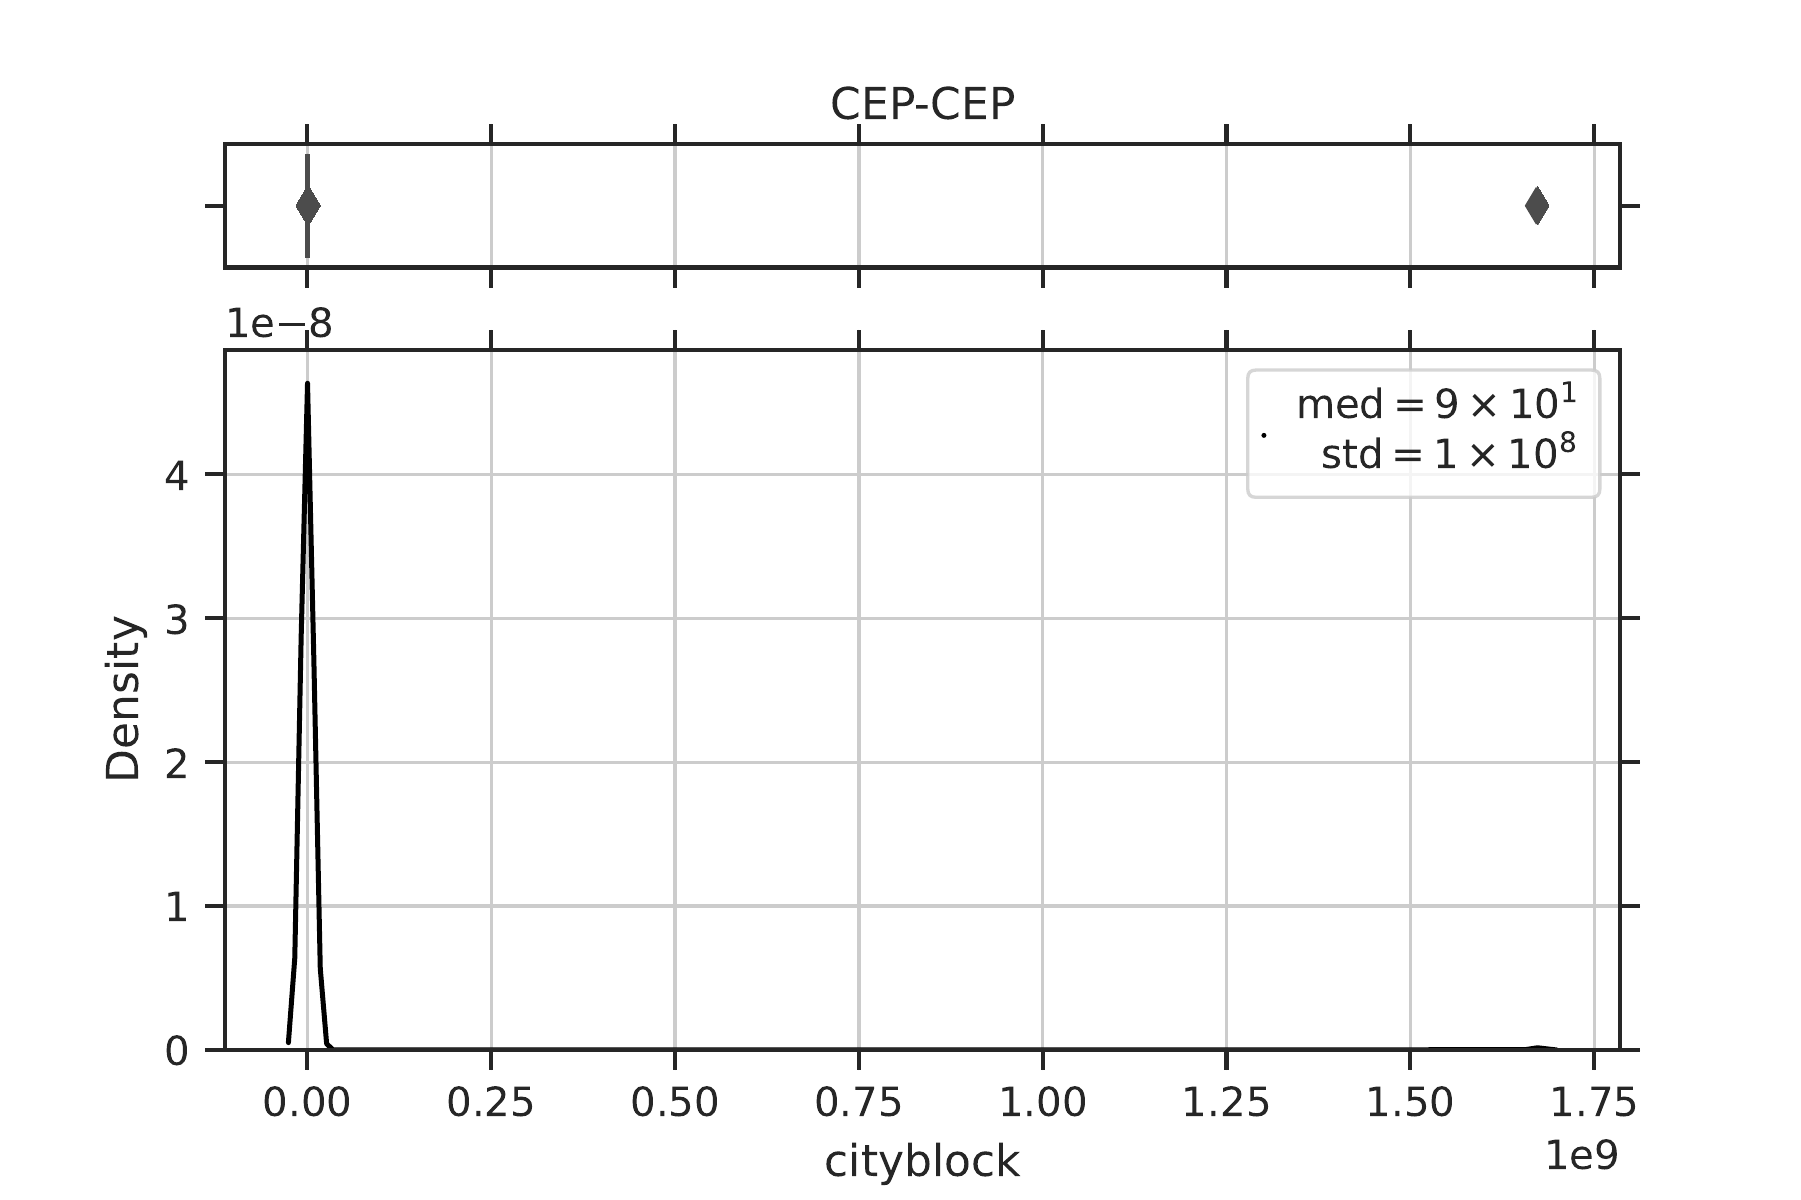
\includegraphics[width=0.49\textwidth]{images/CEP_Before.png}
    }
    \subfloat[After outlier removal]{
        \label{subfig:Cep_after}
        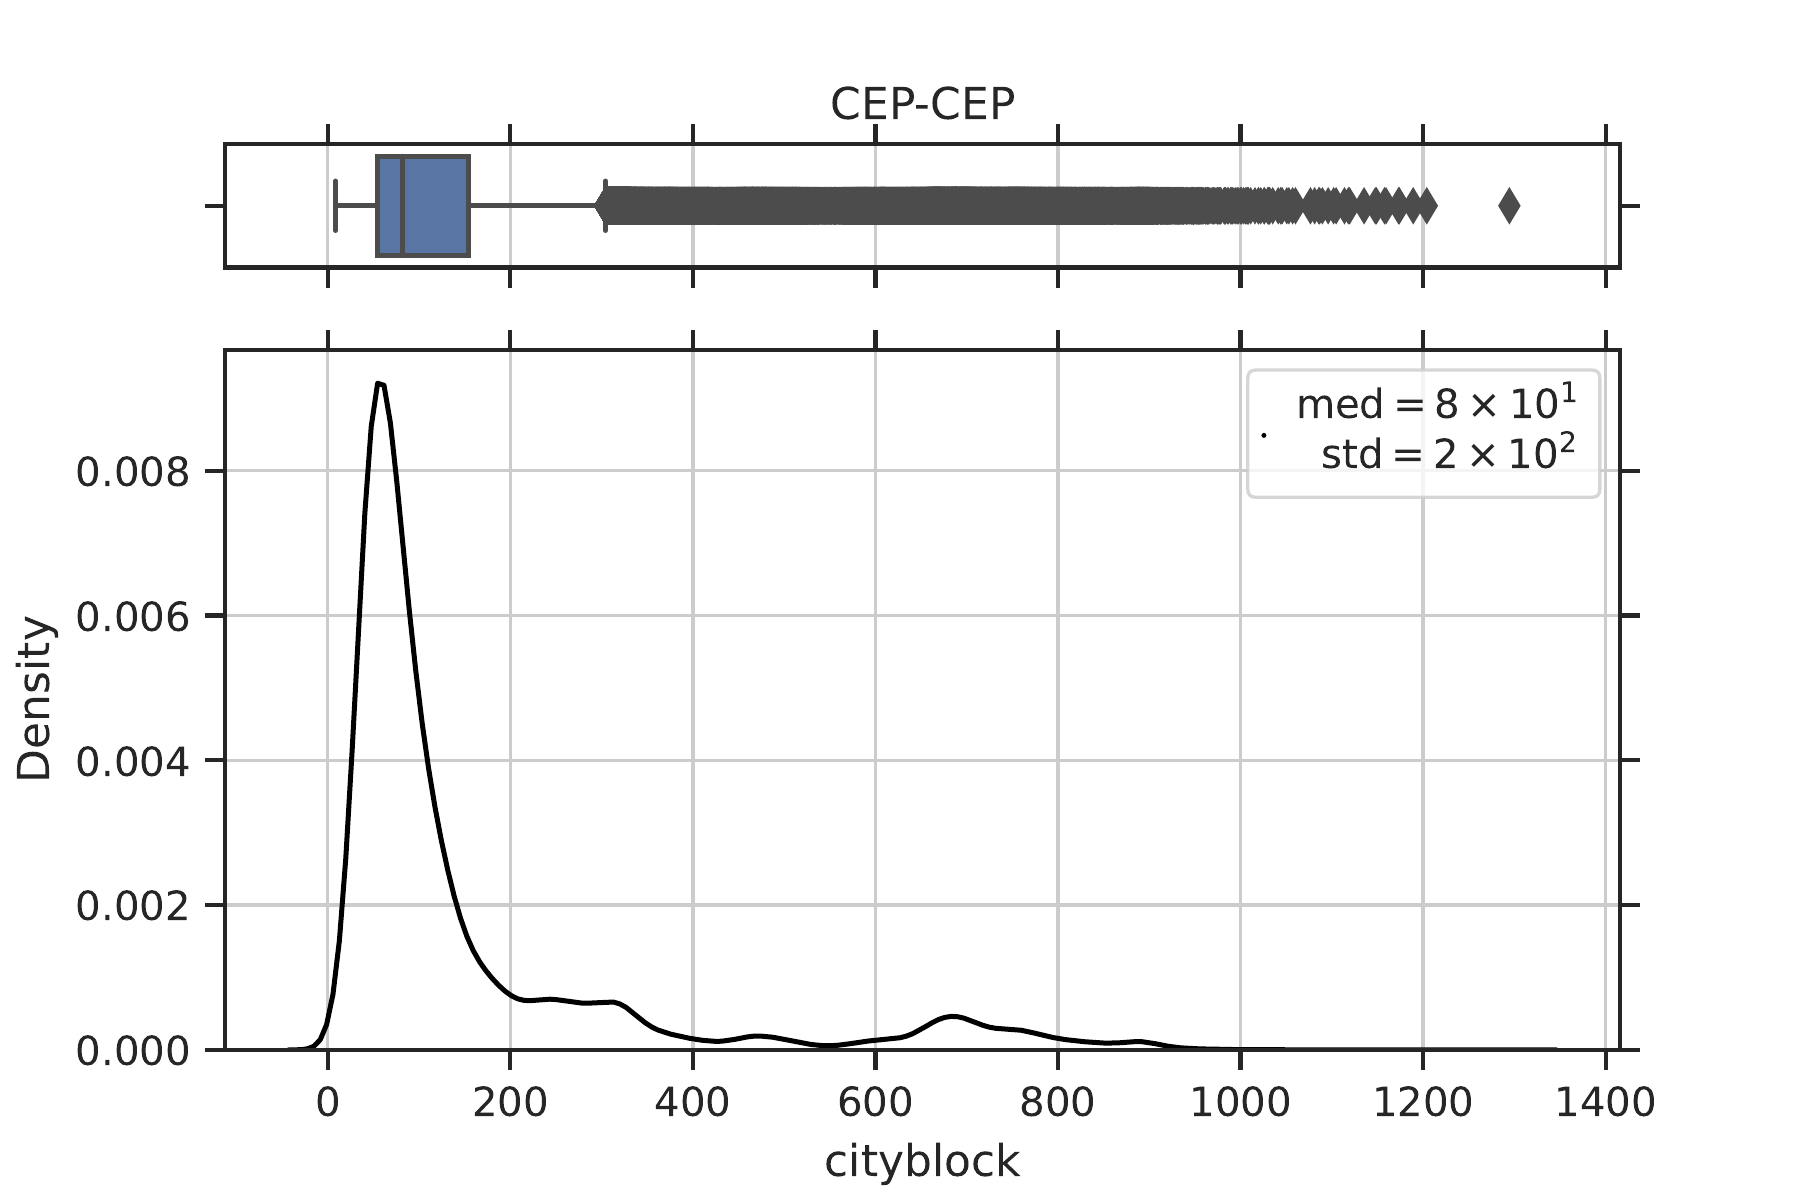
\includegraphics[width=0.49\textwidth]{images/CEP_After.png}
    }
    \caption{Density plot for Cityblock distance distribution between Cepheid variables}
    \label{fig:outlier_removal}
\end{figure*}

Finally, we are left with a `clean' dataset of 558 objects of each class - CEP, RR, RRc, DSCT, Mira, SR, RSCVN, BYDra, EA, EW.

\section{Classification} \label{sec:classification}
%\lipsum[1]

\subsection{Classification Algorithm} \label{subsec:classification_algorithm}
We use a custom algorithm called \texttt{LCDistanceClassifier} to classify the light curves, which is motivated by k-Nearest Neighbours. We implement this on Python using scikit-learn's API \cite{sklearn_api}. We describe our algorithm's training and testing procedure below.
% \note{Maybe add something like https://www.overleaf.com/learn/latex/Algorithms}
\subsubsection{Training}
For all objects in the training set, we calculate the median and the standard deviation per feature per class. The median set represents what an average class's features looks like, and we use it as a representative for each class.

An example of the median set has been displayed in Tab. \ref{tab:median_set}.
\begin{table}[ht]
    \centering
    % \resizebox{0.9\textwidth}{!}{
        \begin{tabular}{|lllll|}
            \hline
            \textbf{Class} & \textbf{\texttt{Period\_band\_r}} & \textbf{\texttt{Amplitude\_r}} & \textbf{\texttt{R21\_r}} & \textbf{\texttt{Skew\_r}} \\ \hline
            CEP            & 3.86                 & 0.25              & 0.27        & -0.16        \\
            RR             & 0.56                 & 0.35              & 0.45        & -0.52        \\
            RRc            & 0.33                 & 0.20              & 0.15        & 0.01         \\
            DSCT           & 0.09                 & 0.08              & 0.17        & -0.14        \\ \hline
            \end{tabular}
% }
\caption{An example of the median set for 4 r-band features and 4 classes.}
\label{tab:median_set}
\end{table}

\subsubsection{Predicting}
To classify a test object, we first choose a distance metric, and then calculate the distance between the test object and the median set for each class from the training step. When calculating the distance, we also scale it by the inverse of the standard deviation for every feature. This step thus tells us how many standard deviations away the test object is from the median set (for a particular metric). This scaling can be denoted by:
% \note{We have illustrated this in Fig. \ref{fig:test_object}.}
\begin{equation} \label{eq:scaling_std_metric}
    d_{\sigma}(u,v)= \sum_{i} \frac{1}{\sigma_i} d_i(u_i,v_i),
\end{equation}
where $i$ denotes the dimension, $d_i$ denotes the $i$th component of the distance metric $d$ in the $i$th dimension and $\sigma_i$ denotes the standard deviation in the $i$th dimension.

Finally, once all the distances have been calculated, we look at the class for which the distance is minimum. This is chosen as the predicted class for a test object. This is then repeated for all test objects to obtain the final class predictions.

\subsubsection{Scoring}
\paragraph{$F_1$ Score}
Once we have made the predictions for all objects in the test set, we measure its performance by calculating the $F_1$ score. The $F_1$ score is given by

\begin{equation} \label{eq:f1_score}
    F_1 = \frac{\text{TP}}{\text{TP} + \frac{1}{2}(\text{FP} + \text{FN})},
\end{equation}
where TP is the number of true positives, FP is the number of false positives, and FN is the number of false negatives. The higher the $F_1$ score, the better the classification, with $100\%$ being the best possible score (all predictions correct) and $0\%$ being the worst possible score (all predictions wrong). For more than two classes, we take the average (\emph{macro} mode) of the $F_1$ scores for each class. Because we consistently maintain class balance, we do not require any weights when calculating the $F_1$ score.

We note that, instead of using a separate training and testing set, we use the cross-validation technique \cite{CrossValidation95}. In this, we split our dataset into 5 parts or 5-folds. We choose four folds as our training set and one fold as our testing set. This is repeated such that all folds are chosen to be the test set exactly once. Finally, we calculate the $F_1$ score for all 5-folds and average the scores to obtain the final score.

\paragraph{Confidence Parameter ($c_p$)}

In addition to the $F_1$ score, we also define a confidence parameter to tell us how confident the prediction by \texttt{LCDistanceClassifier} is.

The confidence parameter, $c_p$, for a prediction is given by

\begin{equation} \label{eq:confidence}
    c_p = \frac{|d_{\text{winner}} - d_{\text{runner-up}}|}{d_{\text{winner}}},
\end{equation}
where $d_{\text{winner}}$ is the distance to the class to which the distance is minimum (the winner is the class that was chosen as the prediction), and $d_{\text{runner-up}}$ is the distance to the class to which the distance is second minimum (the runner-up is the class that would have been chosen had the winner not been present). The confidence parameter thus tells us the relative difference between the distances of the winner and the runner-up. If this difference is large, we then say that the classifier chose the winning class with high confidence and vice versa for low confidence.

For example, if the distance to the winner is $10$ and the distance to the runner up is $100$, then the confidence $c_p = \frac{100-10}{10} = 9$. On the other hand, if the distance to the winner is $99$ and the distance to the runner up is $100$, then the confidence $c_p = \frac{100-99}{99} = 0.01$.

The motivation behind having the confidence values is that they serve as an additional measure of the quality of the classification. A high $F_1$ score implies that the predictions made by our classifier are correct and agree with \cite{chenZwickyTransientFacility2020a}'s catalog. In contrast, high confidence tells us that the classifier is confident about its prediction. Ideally, a perfect classifier would have a $F_1$ score of $100\%$ with a high confidence value for each prediction. Thus, by choosing the classifier with the top $F_1$ score followed by the highest confidence value, we can determine which distance metric is the best for a given classification problem.


\section{Feature Selection and Dimensionality Reduction} \label{sec:feature_selection}

To reduce the dimensionality of the feature space, we employ the Forward Sequential Feature Selection strategy \cite{ferriComparativeStudyTechniques1994} with \texttt{LCDistanceClassifier}. We start by choosing the single feature (from the 118) that maximises our 5-fold cross-validation $F_1$ score with just that feature. Once we have selected this, we then choose the next feature, which, when added to the feature set, maximises the 5-fold cross-validation $F_1$. We repeat this process until we have selected all of the 118 features. The total number of combinations are thus,

\begin{align}
    \text{No. of combinations} &= \sum_{i=0}^{n} \binom{n-i}{1} \notag \\
    % &=\binom{n}{1}+\binom{n-1}{1}+\binom{n-2}{1}+...+\binom{1}{1} \notag \\
    % &=\frac{n!}{(n-1)!\ 1!}+\frac{(n-1)!}{(n-2)!\ 1!}+\frac{(n-2)!}{(n-3)!\ 1!}+...+\frac{1!}{0!\ 1!} \notag \\
    % &=n+(n-1)+(n-2)+...+1 \notag \\
    &=\frac{n(n+1)}{2} \label{eq:tot_sfs_calcs}\\
    &=\mathcal{O}(n^2) \label{eq:bigo_sfs}
\end{align}

Here, because $n=118$, we perform a total of $7021$ calculations for each metric for a classification problem.

Thus, this gives us the order of importance of the features for a particular classification problem - the feature selected first has the highest importance, while the feature selected last has the least importance. In addition, the Sequential Feature Selection strategy also allows us to find out how the performance changes with the number of features included. Finally, once we know the small set of most important features, we can drop the remaining unimportant features to reduce the dimensionality of our feature space.

Because each metric and class behaves differently, we expect the top features to depend on both the classification problem, as well as the metric used. We present our results for this in detail in the next section \ref{sec:results}.

\section{Results} \label{sec:results}
%\lipsum[2-4]

\section*{Acknowledgment}

% The preferred spelling of the word ``acknowledgment'' in America is without 
% an ``e'' after the ``g''. Avoid the stilted expression ``one of us (R. B. 
% G.) thanks $\ldots$''. Instead, try ``R. B. G. thanks$\ldots$''. Put sponsor 
% acknowledgments in the unnumbered footnote on the first page.

%%%%%%%%%%%%%%%%%%%%%%%%%%%%%%%%%%%%%%%%%%%%%%%%%%

%%%%%%%%%%%%%%%%%%%% REFERENCES %%%%%%%%%%%%%%%%%%

% The best way to enter references is to use BibTeX:

%\bibliographystyle{mnras}
%\bibliography{example} % if your bibtex file is called example.bib


% Alternatively you could enter them by hand, like this:
% This method is tedious and prone to error if you have lots of references

\bibliographystyle{IEEEtran}
\bibliography{mybib,mybib_new,alercebibs}

\appendix

\subsection{Distance Metric Definitions} \label{app:metrics}
\begin{defn} \label{def:distance}
The distance d between two points, in a set X, is a function $ d: X \times X \rightarrow [0, \infty)$ that gives a distance between each pair of points in that set such that, for all $x,y,z \in X$, the following properties hold:
\begin{enumerate}
\item $d(x,y) = 0 \iff x = y$ (identity of indiscernibles)
\item $d(x,y) = d(y,x)$ (symmetry)
\item $d(x,y) \leq d(x,z) + d(z,y)$ (triangle inequality)
\end{enumerate}
\end{defn}

\begin{cor}
From the above three axioms, the following condition also holds:
\begin{equation}
d(x,y) \geq 0, \text{for all } x,y \in X
\end{equation}
\end{cor}

\begin{exmp}
The Euclidean distance between two points in $\mathbb{R}^2$ is an example of a distance. Similarly, we can define a distance between any set of points such that the definition \ref{def:distance} is satisfied.
\end{exmp}

\begin{defn} \label{def:metric_space}
A metric space $(X,d)$ is a set $X$ equipped with a metric $d$.
\end{defn}

\begin{exmp}
The 2-dimensional $\mathbb{R}^2$ plane with the Euclidean distance is an example of a metric space.  Similarly, we can also define metrics on matrices, functions, sets of points or any other mathematical object as long as it satisfies the definition \ref{def:metric_space}.
\end{exmp}

Now, we note the difference between the terms \emph{distance} and \emph{distance metric} (often shortened to just \emph{metric}).
\begin{defn}
The term \emph{metric} refers to the way of computing the distance between any two elements of the set. Meanwhile, the term \emph{distance} refers to the scalar value obtained after using a particular metric on a pair of elements in the set.
\end{defn}

\begin{exmp}
The Euclidean metric for $\mathbb{R}^2$ is given by $ d = \sqrt{(x_2 - x_1)^2 + (y_2 - y_1)^2} $, while the Euclidean distance between the points $(0,0)$ and $(1,1)$ is given by $ d = \sqrt{2} $.
\end{exmp}

\subsection{List of Metrics} \label{app:list_of_metrics}
We used the following metrics for all distance calculations in this paper. For a detailed description of each metric, see \cite{dezaEncyclopediaDistances2013}.
\begin{enumerate}
    \item \textbf{Euclidean metric}:\\
    \begin{equation} \label{eq:euclidean_metric}
        d(u,v)=\sqrt{\sum \big(v_i - u_i\big)^2}
    \end{equation}
    The Euclidean metric is the most widely used metric, and represents the length of the shortest straight line joining 2 points.

    \item \textbf{Cityblock metric}:\\
    \begin{equation} \label{eq:cityblock_metric}
        d(u,v)={\sum\big|v_i - u_i\big|}
    \end{equation}
    The Cityblock metric gives the shortest path between 2 points if we restrict movement to the grid. Named after the grid layout of cities, this is the shortest distance for a taxi to traverse between two places. It is also known as the Manhattan metric.

    \item \textbf{Bray-Curtis metric}:\\
    \begin{equation} \label{eq:bray_curtis_metric}
        d(u,v)=\dfrac{\sum\left|u_{i}-v_{i}\right|}{\sum\left|u_{i}+v_{i}\right|}
    \end{equation}
    The Bray-Curtis metric is a modified version of the Cityblock metric. Note that the summation is performed independently on the numerator and denominator before division.

    \item \textbf{Canberra metric}:\\
    \begin{equation} \label{eq:canberra_metric}
        d(u, v)=\sum_{i} \frac{\left|u_{i}-v_{i}\right|}{\left|u_{i}\right|+\left|v_{i}\right|}
    \end{equation}
    The Canberra metric is another modified version of the Cityblock metric, whose denominator is slightly different from the Bray-Curtis metric.

    \item \textbf{Chebyshev metric}:\\
    \begin{equation} \label{eq:chebyshev_metric}
        d(u,v)=\max\big(|u_i-v_i|\big)
    \end{equation}
    The Chebyshev metric is also known as the chessboard metric. It represents the minimum number of moves needed by the King chess piece to move from one point to another.

    \item \textbf{Correlation metric}:\\
    \begin{equation} \label{eq:correlation_metric}
        d(u,v)=1-\frac{(u-\bar{u}) \cdot(v-\bar{v})}{\|(u-\bar{u})\|_{2}\|(v-\bar{v})\|_{2}}
    \end{equation}
    The Correlation metric is based on the Pearson correlation coefficient between 2 points, it is given by:

    \item \textbf{Cosine metric}:\\
    \begin{equation} \label{eq:cosine_metric}
        d(u,v)=\frac{\sum\left(u_{i}-\bar{u})\cdot(v_{i}-\bar{v})\right)}{\sqrt{\sum\left(u_{i}-\bar{u})\cdot(u_{i}-\bar{u})\right)}\sqrt{\sum\left(v_{i}-\bar{v})\cdot(v_{i}-\bar{v})\right)}}
    \end{equation}
    The Cosine metric is based on the cosine similarity, which depends only on the angle between two vectors and not their magnitude.

    \item \textbf{Soergel metric}:\\
    \begin{equation} \label{eq:soergel_metric}
        d(u,v)=\frac{\sum\left|u_{i}-v_{i}\right|}{\sum \max \left\{u_{i}, v_{i}\right\}}
    \end{equation}
    The Soergel metric is another modified version of the Cityblock metric but only has a $\max$ term in the denominator. Note that the summation is performed independently on the numerator and denominator before division.

    \item \textbf{Kulczynski metric}:\\
    \begin{equation} \label{eq:kulczynski_metric}
        d(u,v)=\frac{\sum\left|u_{i}-v_{i}\right|}{\sum \min \left\{u_{i}, v_{i}\right\}}
    \end{equation}
    The Kulczynski metric is similar to the Soergel metric, with the difference that its denominator consists of a minimum instead of a maximum.

    \item \textbf{Wave–Edges metric}:\\
    \begin{equation} \label{eq:wave_edges_metric}
        d(u,v)=\sum \frac{\left|u_{i}-v_{i}\right|}{\max \left\{u_{i}, v_{i}\right\}}
    \end{equation}
    The Wave-Edges metric is a slight modification of the Soergel metric, where the summation is done after division.

    \item \textbf{Jaccard metric}:\\
    \begin{equation} \label{eq:jaccard_metric}
        d(u,v)=\frac{\left(\sum u_{i}-v_{i}\right)^{2}}{\sum u_{i}^{2}+\sum v_{i}^{2}-\sum u_{i} v_{i}}
    \end{equation}
    The Jaccard metric is based on the Jaccard similarity coefficient, which is a measure of similarity between 2 sets.

    \item \textbf{Maryland Bridge metric}:\\
    \begin{equation} \label{eq:maryland_bridge_metric}
        d(u,v)=1-\frac{1}{2}\left(\frac{\sum u_{i} v_{i}}{\sum u_{i}^{2}}+\frac{\sum u_{i} v_{i}}{\sum v_{i}^{2}}\right)
    \end{equation}
    The Maryland-Bridge metric is based on the Maryland Bridge similarity.

    \item \textbf{Motyka metric}:\\
    \begin{equation} \label{eq:motyka_metric}
        d(u,v)=\frac{\sum \max \left\{u_{i}, v_{i}\right\}}{\sum\left(u_{i}+v_{i}\right)}
    \end{equation}
    Unlike the previous metrics, the Motyka metric has a maximum term in the numerator and a summation term in the denominator.

    \item \textbf{Lorentzian metric}:\\
    \begin{equation} \label{eq:lorentzian_metric}
        d(u,v)=\sum \ln \left(1+\left|u_{i}-v_{i}\right|\right)
    \end{equation}
    Because the Lorentzian metric is given by a natural log, it is more sensitive to changes in the input vectors, as the log blows up quickly.

    \item \textbf{Clark metric}:\\
    \begin{equation} \label{eq:clark_metric}
        d(u,v)=\left(\frac{1}{n} \sum\left(\frac{u_{i}-v_{i}}{\left|u_{i}\right|+\left|v_{i}\right|}\right)^{2}\right)^{\frac{1}{2}}
    \end{equation}
    The Clark metric can be thought of as a combination of the Euclidean metric and the Canberra metric, where the ratio is similar to the Canberra metric, which is squared, summed and taken a square root of, like the Euclidean metric.

    \item \textbf{Meehl metric}:\\
    \begin{equation} \label{eq:meehl_metric}
        d(u,v)=\sum_{1 \leq i \leq n-1}\left(u_{i}-v_{i}-u_{i+1}+v_{i+1}\right)^{2}
    \end{equation}
    The Meehl metric mixes terms from consecutive dimensions, thus making the ordering of the dimensions significant.

    \item \textbf{Hellinger metric}:\\
    \begin{equation} \label{eq:hellinger_metric}
        d(u,v)=\sqrt{2 \sum\left(\sqrt{\frac{u_{i}}{\bar{u}}}-\sqrt{\frac{v_{i}}{\bar{v}}}\right)^{2}}
    \end{equation}
    The Hellinger metric is a metric that is commonly used to compare two probability distributions but can also be used with numeric data.

    \item \textbf{Symmetric $\chi^2$ metric}:\\
    \begin{equation} \label{eq:symmetric_chi_2_metric}
        d(u,v)=\sqrt{\sum \frac{\bar{u}+\bar{v}}{n(\bar{u} \cdot \bar{v})^{2}} \cdot \frac{\left(u_{i} \bar{v}-v_{i} \bar{u}\right)^{2}}{u_{i}+v_{i}}}
    \end{equation}
    The symmetric $\chi^2$ metric is a kind of a weighted Euclidean metric, where terms between the two vectors are mixed.
\end{enumerate}

\end{document}
